\documentclass{beamer}

% \usepackage{beamerthemesplit} // Activate for custom appearance

\title{The Sequence Memoizer}
\author{Frank Wood\newline\newline fwood@stat.columbia.edu \newline\newline {\small Joint work with Jan Gasthaus, C\'{e}dric  Archambeau, Lancelot James, and Yee Whye Teh}}
\date{\today}

\newcommand{\comment}[1]{}
\newcommand{\ponedec}{\mathcal{P}^\downarrow_1}
\newcommand{\pone}{\mathcal{P}_1}
\newcommand{\rank}[1]{\mathrm{RANK}\left[#1\right]}
\newcommand{\E}[1]{\mathrm{E}\left[#1\right]}
\newcommand{\py}{\mathcal{PY}}
\newcommand{\iid}{iid.}
\newcommand{\drawiid}{\stackrel{\text{iid}}{\sim}}
\newcommand{\vect}[1]{\mathbf{#1}}
\newcommand{\indicator}[1]{\text{I}\left[ #1 \right]}
\newcommand{\pdcoag}{PD(d_1,0)-\text{COAG}}
\newcommand{\todo}{\textbf{*TODO*}}
\newcommand{\igram}{\text{$\infty$-gram}}
\newcommand{\Prob}{\text{P}}

\def\mm{sequence memoizer }
\def\MM{SM }

\def\pibf{{\boldsymbol{\pi}}}
\def\kapbf{\boldsymbol{\kappa}}
\def\taubf{\boldsymbol{\tau}}
\def\thebf{\boldsymbol{\theta}}
\def\rhobf{\boldsymbol{\rho}}
\def\phibf{\boldsymbol{\phi}}
\def\pbf{\mathbf{p}}
\def\qbf{\mathbf{q}}
\def\sbf{\mathbf{s}}
\def\tbf{\mathbf{t}}
\def\ybf{\mathbf{y}}
\def\ubf{\mathbf{u}}

\def\wbf{\mathbf{w}}
\def\xbf{\mathbf{x}}
\def\rbf{\mathbf{r}}
\def\tbf{\mathbf{t}}
\def\kbf{\mathbf{k}}
\def\Xbf{\mathbf{X}}
\def\0bf{\mathbf{0}}
\def\Ibf{\mathbf{I}}
\def\phibf{\mathbf{\phi}}
\def\Phibf{\mathbf{\Phi}}
\def\disteq{{\stackrel{D}{=}}}
\def\EE{{\mathbb{E}}}
\def\GG{\mathcal{G}}

\def\phiv{\varphi}
\def\phivbf{\boldsymbol{\varphi}}

\def\Ocal{\mathcal{O}}

\DeclareMathOperator*{\Bet}{Beta}
\DeclareMathOperator{\coag}{COAG}
\DeclareMathOperator{\frag}{FRAG}
\DeclareMathOperator*{\rnk}{RANK}
\DeclareMathOperator*{\gem}{GEM}
\DeclareMathOperator*{\pd}{PD}
\DeclareMathOperator*{\gd}{GDir}
\DeclareMathOperator*{\Dir}{Dir}
\DeclareMathOperator*{\argmax}{argmax}


\begin{document}

\frame{\titlepage}

\section[Outline]{}
\frame{\tableofcontents}



\section{Sequence Modeling}
\subsection{Example Applications}
\subsection{Theory}

\frame[t] {%slide 1
 \frametitle{Executive Summary}
 Sequence Memoizer (SM) \cite{wood2009sms}
\begin{itemize}
\item ``Joint,'' ``non-Markov'' model of discrete sequences 
\item Efficient (linear space, worst case quadratic time) estimation algorithm
\item Drop in replacement for $n^{th}$ order Markov model.
\item Full context always used in inference
\end{itemize}

Name describes mechanics of posterior inference algorithm \cite{Goodman:UAI08}
}
\frame[t] {%slide 1.5
 \frametitle{Executive Summary}
 Example Applications
\begin{itemize}
\item Language modeling
\begin{itemize}
\item Computational cost of 5-gram on non-antagonistic data
\item Inference in (SM) is limit of $n$-gram as $n\rightarrow\infty$
\end{itemize}
\item Compression
\begin{itemize}
\item Competitive with context tree weighting (CTW) \cite{ctwresults} and unbounded context prediction by partial matching (PPM) \cite{cleary95unboundedlength,cleary1984dca, moffat1990ipd} variants
\end{itemize}
\end{itemize}
 }
\frame[t] {%slide 2
 \frametitle{Inspiration}
 ``Prediction and entropy of printed English,'' \cite{shannon1950}
\begin{quote}
If $[\ldots]$ language is translated into binary digits $[\ldots]$, the entropy H $[\mbox{of the language}]$ is the average number of binary digits required per letter
\end{quote} 
{\begin{center} drppng lttrs dsnt hrt \end{center} }
\begin{quote} $[\ldots]$it appears that, in ordinary literary English, $[\ldots]$ long range statistical effects (up to 100 letters) reduce the entropy to something of the order of one bit per letter
\end{quote}
{\begin{center} d \_ \end{center} }
{\begin{center} the united \_ \end{center} }
{\begin{center} baseball is the national pastime of the united \_ \end{center} }

 }
 \frame[t] {%slide 3
 \frametitle{Inspiration and Reminder}
 Conclusion: lower and upper bound on character-based entropy of English of
$[0.6 < H(English) < 1.3]$ bits per character\footnote{based on a 27 character alphabet, where $log_2(27) \approx 4.75$} \cite{shannon1950}
 \newline
 
 If $\Sigma$ is a set (an alphabet) and $G$ is a discrete probability distribution over $\Sigma$, (i.e. $\sum_{x\in\Sigma} G(X=x) = 1, 0 < G(x) < 1)$ then you can write the entropy of $G$ as
 
 \[H(G) = -\sum_{x\in\Sigma} G(x) \log_2(G(x))\]
 
 Reminder: entropy is the number of bits per symbol an optimal encoder of a sequence of iid symbols drawn from $G$ would require to losslessly represent the sequence on average. 
 
 }
 \frame[t] {%slide 4
 \frametitle{Crazy Idea}
 \begin{center}Compression $\approx$ intelligence\end{center}
 ``Text Compression as a Test for Artificial Intelligence,''\cite{largetext} \newline
 
\begin{quote}The Turing test for artificial intelligence is widely accepted, but is subjective, qualitative, non-repeatable, and difficult to implement. An alternative test without these drawbacks is to insert a machine's language model into a predictive encoder and compress a corpus of natural language text. A ratio of 1.3 bits per character or less indicates that the machine has AI.\end{quote}
 }
 \frame[t] {%slide 5
 \frametitle{Of Mouths and Money}
 The (Marcus) Hutter prize \cite{hutter} \newline
 
\begin{quote}Wikipedia is an extensive snapshot of Human Knowledge. If you can compress the first 100MB of Wikipedia better than your predecessors, your (de)compressor likely has to be smart(er). The intention of this prize is to encourage development of intelligent compressors/programs.
 \end{quote}
 \begin{itemize}
\item 50,000 euro in prize money available
\item http://prize.hutter1.net/ 
 \end{itemize}
 }

 \frame[t] {%slide 6
 \frametitle{Sequence Data}
 \begin{itemize}
\item  Natural language processing 
 \begin{itemize}
\item Words, i.e.~the united \_
\item Characters, i.e.~un\_
\item Parts of speech, i.e.~NNV\_
\end{itemize}
\item Compression 
 \begin{itemize}
\item  Bits i.e.~0101000011110001\_
\item  Bytes i.e.~6A7B4ED22100D\_
\end{itemize}
\item Computational biology 
 \begin{itemize}
\item  Nucleotides i.e.~actgtc\_
\item Genes
\item ...
\end{itemize}
\item ...
\end{itemize}

 }
 \frame[t] {%slide 7
 \frametitle{Example Applications}
 \begin{itemize}
 \item Filling in missing segments
 \[ \argmax_{x_1, x_2, \ldots, x_k} P(010010x_1 x_2 x_3 \ldots x_k 010) \]
 \item Predict what comes next in the sequence 
  \[ \argmax_{x_{i+1}} P(010010010x_{i+1}) \]
 \item Determine typicality (clustering)
   \[ \argmax_{k} P_k(010010010) \]

 \end{itemize}
 }
 \frame[t] {%slide 8
 \frametitle{The Sequence Memoizer}
 The sequence memoizer is a regularized (Bayesian\footnote{$P(data,parameters) = P(parameters)P(data|parameters)$}) model of sequences.  \newline
\begin{align}
P(\xbf,\GG) = P(\GG)\prod_{i=0}^{|\xbf|-1}G_{\xbf_{1:i}}(\xbf_{i+1}) \nonumber
\end{align}
The sequence memoizer represents the joint distribution of a sequence in terms of a product of conditional distributions.  If the probability of each
symbol $s$ following each context $\ubf$ is given by a latent variable (distribution) $G_\ubf(s)$ then

\begin{align}
P(\xbf|\GG) = G_{\{\}}(x_{1})G_{x_1}(x_{2})G_{\xbf_{1:2}}(x_{3})\cdots G_{\xbf_{1:(|\xbf|-1)}}(x_{|\xbf|})  \nonumber 
\end{align}

The resulting likelihood is, by definition, a ``joint''\footnote{$P(x_1,\ldots,x_i|\theta) = P(x_1|\theta) P(x_2 | x_1, \theta) P(x_3 | x_1,x_2, \theta) \cdots P(x_i | \xbf_{1:(i-1)}, \theta)$} likelihood.

 }
 \frame[t] {%slide 9
 \frametitle{The Crux of the Matter}
 Can we learn a joint distribution of over sequences of unbounded length given a single training sequence? (!!!) \newline
 
 \quad Obviously not without strong regularization.  \newline
 
 With Bayesian regularization we can do posterior inference of the following flavor
 
 \[P(x_{i+1} | \xbf_{1:i}) = \int G_{\xbf_{1:i}}(x_{i+1}) dP(G_{x_{i+1} }|\xbf_{1:i}) \]
 
 or more recognizably (but less accurately)
 
 \[P(x_{i+1} | \xbf_{1:i}) = \int P(x_{i+1} | \xbf_{1:i}, \GG) P(\GG | \xbf_{1:i}) d\GG \]

 
 
 }
  \frame[t] {%slide 9.5
 \frametitle{Big Picture}
 The sequence memoizer draws on a diverse set of prior art
 \begin{itemize}
 \item A structured prior on the collection of all conditional probability distributions $\GG$, $P(\GG)$
   \begin{itemize}
   \item Hierarchical Pitman Yor process \cite{Teh:JASA06, goldwaterj06, Teh:ACL06}
   \end{itemize}
 \item A method for drawing samples from $P(\GG|\xbf)$
    \begin{itemize}
   \item Chinese restaurant franchise sampler \cite{Teh:JASA06}
   \end{itemize}
 \item A collection of methods for collapsing the the posterior down to a size that grows linearly in the length of the observation sequence. 
    \begin{itemize}
   \item Coagulation and fragmentation operators \cite{Pitman1999, HoJames}
   \end{itemize}
 \item A set of algorithms to identify the remaining graphical model.
   \begin{itemize}
   \item Suffix tree construction \cite{Weiner:IEEE73,Ukkonen:ASAIP92}
   \end{itemize}
 \end{itemize}
  }
  
 \frame[t] {%slide 10
 \frametitle{History - statistically modeling sequences}
 Take a long sequence
 \begin{quote}
 aaaaagagaaaagaaaagactgggaaaagcgcgcgcgc...
 \end{quote}
 Pick a order for a Markov model (here 2).  Train the Markov model by counting.
 \[G_{aa}(x) = \frac{\#\{aax\}}{\#\{aa\}}, G_{aa}(g) = \frac{4}{13}\]
Problems
 \begin{itemize}
\item Short order Markov models can't capture long range dependencies
\item High order Markov models have many parameters, $O(|\Sigma|^n)$.
 \begin{itemize}
 \item Don't know if $G_{aa}(c) = 0$ or just not enough data seen yet.
 \item $G_{\ubf}(x) = 0$ causes all sorts of inference problems.
 \item Regularization of some form is imperative.
 \end{itemize}
\end{itemize}
 }

\frame[t] {%slide 11
 \frametitle{Reasonable regularizations}
 In many real life sequential generative processes it is reasonable to believe that 
 \[G_{\ubf}(s) \approx G_{\sigma(\ubf)}(s)\]
 Where $\sigma(x_1x_2x_3\ldots x_n) = x_2x_3\ldots x_n$ is the suffix operator.  For example
 \[G_{adl}(y) \approx G_{dl}(y)\]
 or really just 
  \[G_{\ubf} \approx G_{\sigma(\ubf)}\]

 }
\frame[t] {%slide 12
 \frametitle{Language Modeling}
 Smoothing and interpolating n-gram models have utilized this intuition for many years \cite{kneser1995ibo,mackayp95,Chen:CSL99, goldwaterj06, Teh:ACL06} \newline
 
 All of these models can be expressed in forms similar to
 
   \[G_{\ubf}(s) \propto \frac{\#\{\ubf s\}}{\#\{\ubf\}} + \lambda G_{\sigma(\ubf)}(s)\]

 Predictive models for compression also utilize predictive distributions of similar form \cite{ctwbasic, cleary1984dca}
 }
 \frame[t] {%slide 13
 \frametitle{}
 }
 \frame[t] {%slide 14
 \frametitle{}
 }
 \frame[t] {%slide 15
 \frametitle{}
 }
 \frame[t] {%slide 16
 \frametitle{}
 }
 \frame[t] {%slide 17
 \frametitle{}
 }
 \frame[t] {%slide 18
 \frametitle{}
 }
 \frame[t] {%slide 19
 \frametitle{}
 }
 \frame[t] {%slide 20
 \frametitle{$O(n^2)$ graphical model}
 \begin{figure}[htbp]
\begin{center}
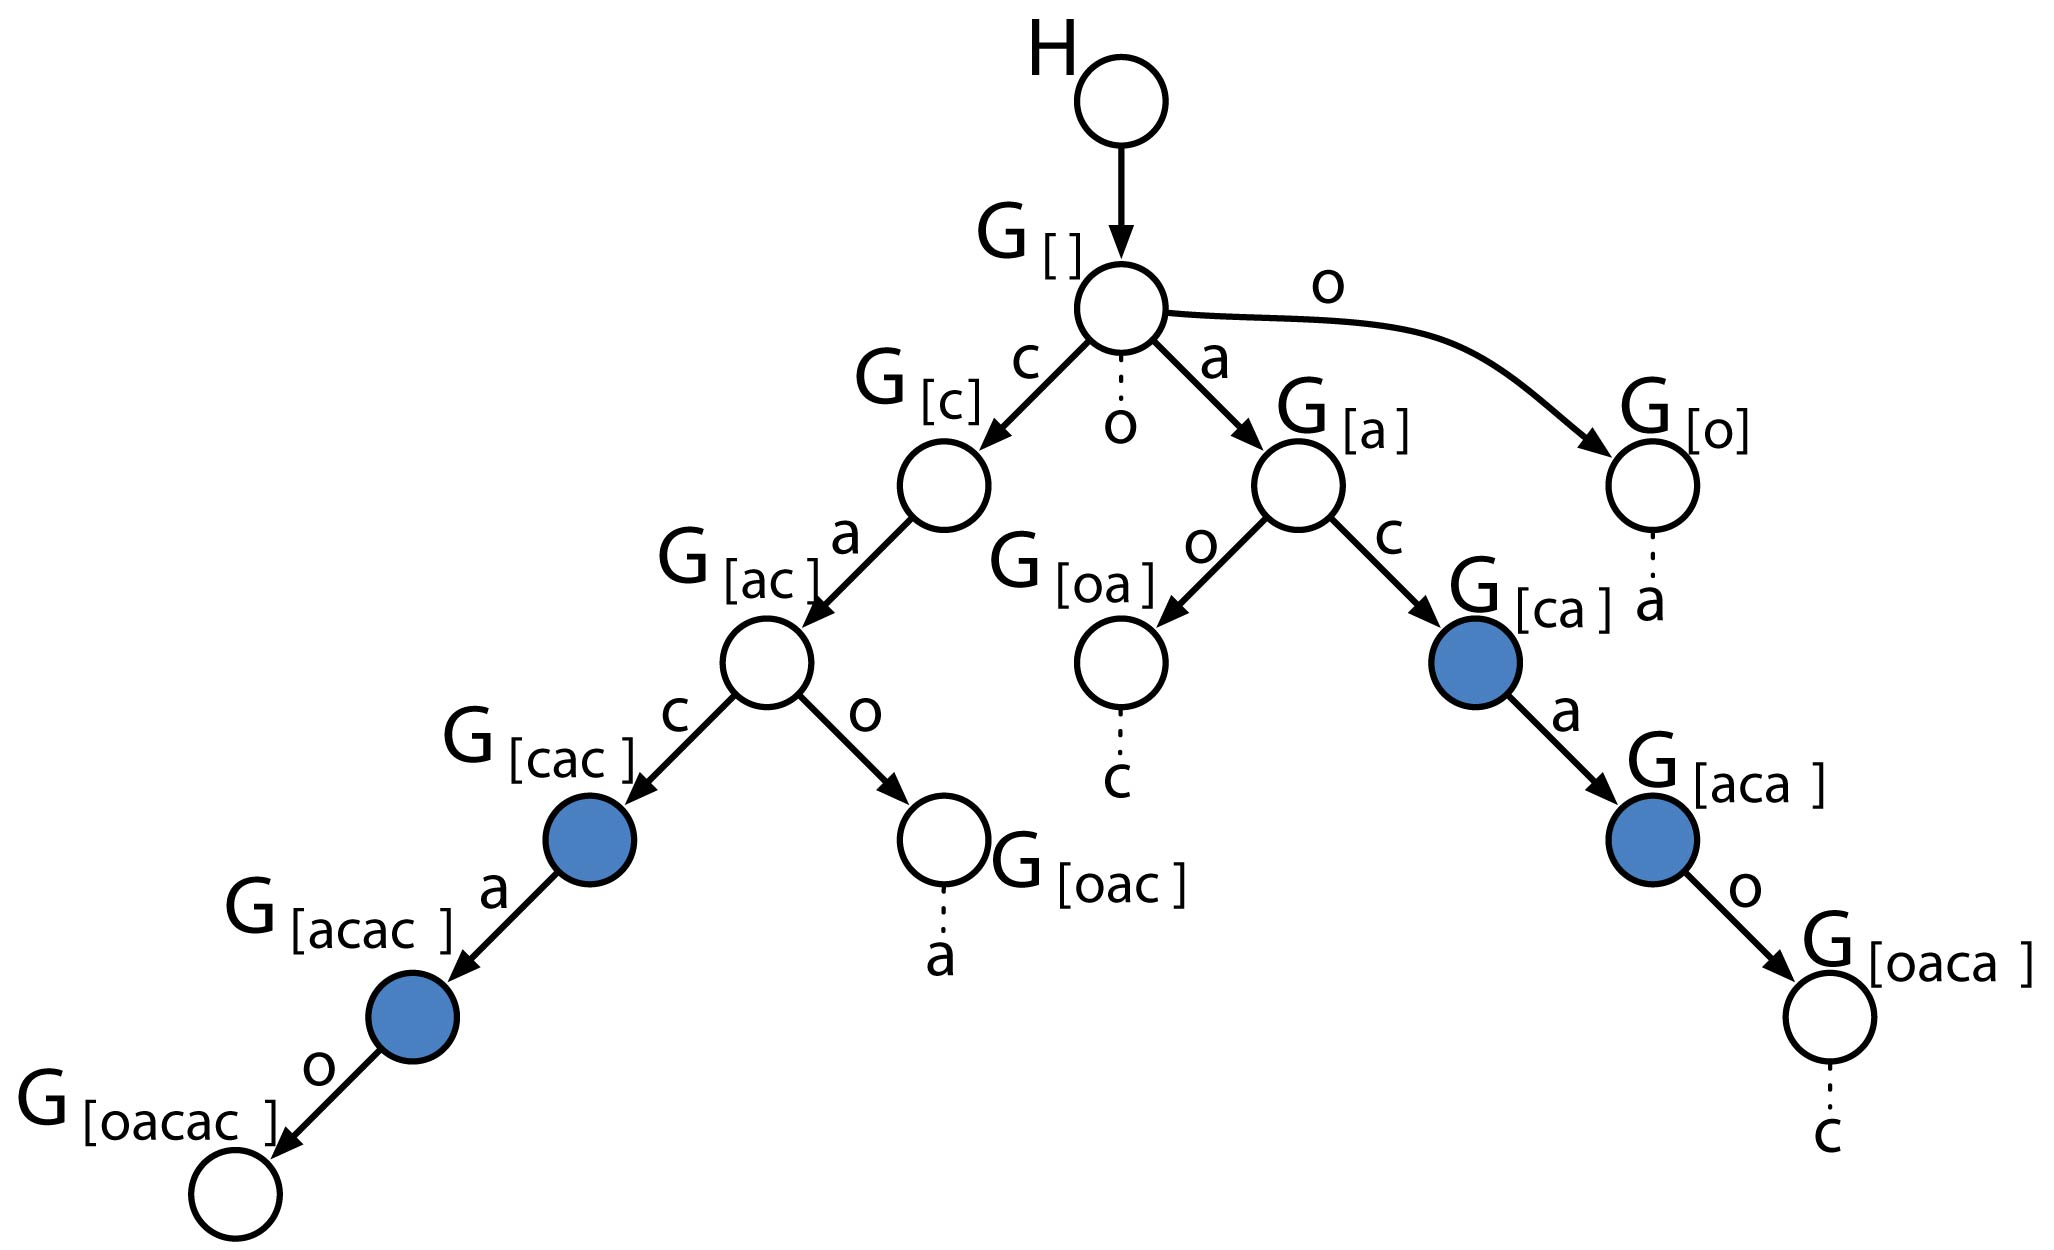
\includegraphics[width=.5\textwidth]{fig/prefix_trie_coloured.pdf}
\caption{Prefix {\em trie} graphical model}
\label{fig: prefix_trie}
\end{center}
\end{figure}
 }
 \frame[t] {%slide 21
\frametitle{$O(n)$ graphical model}
 \begin{figure}[htbp]
\begin{center}
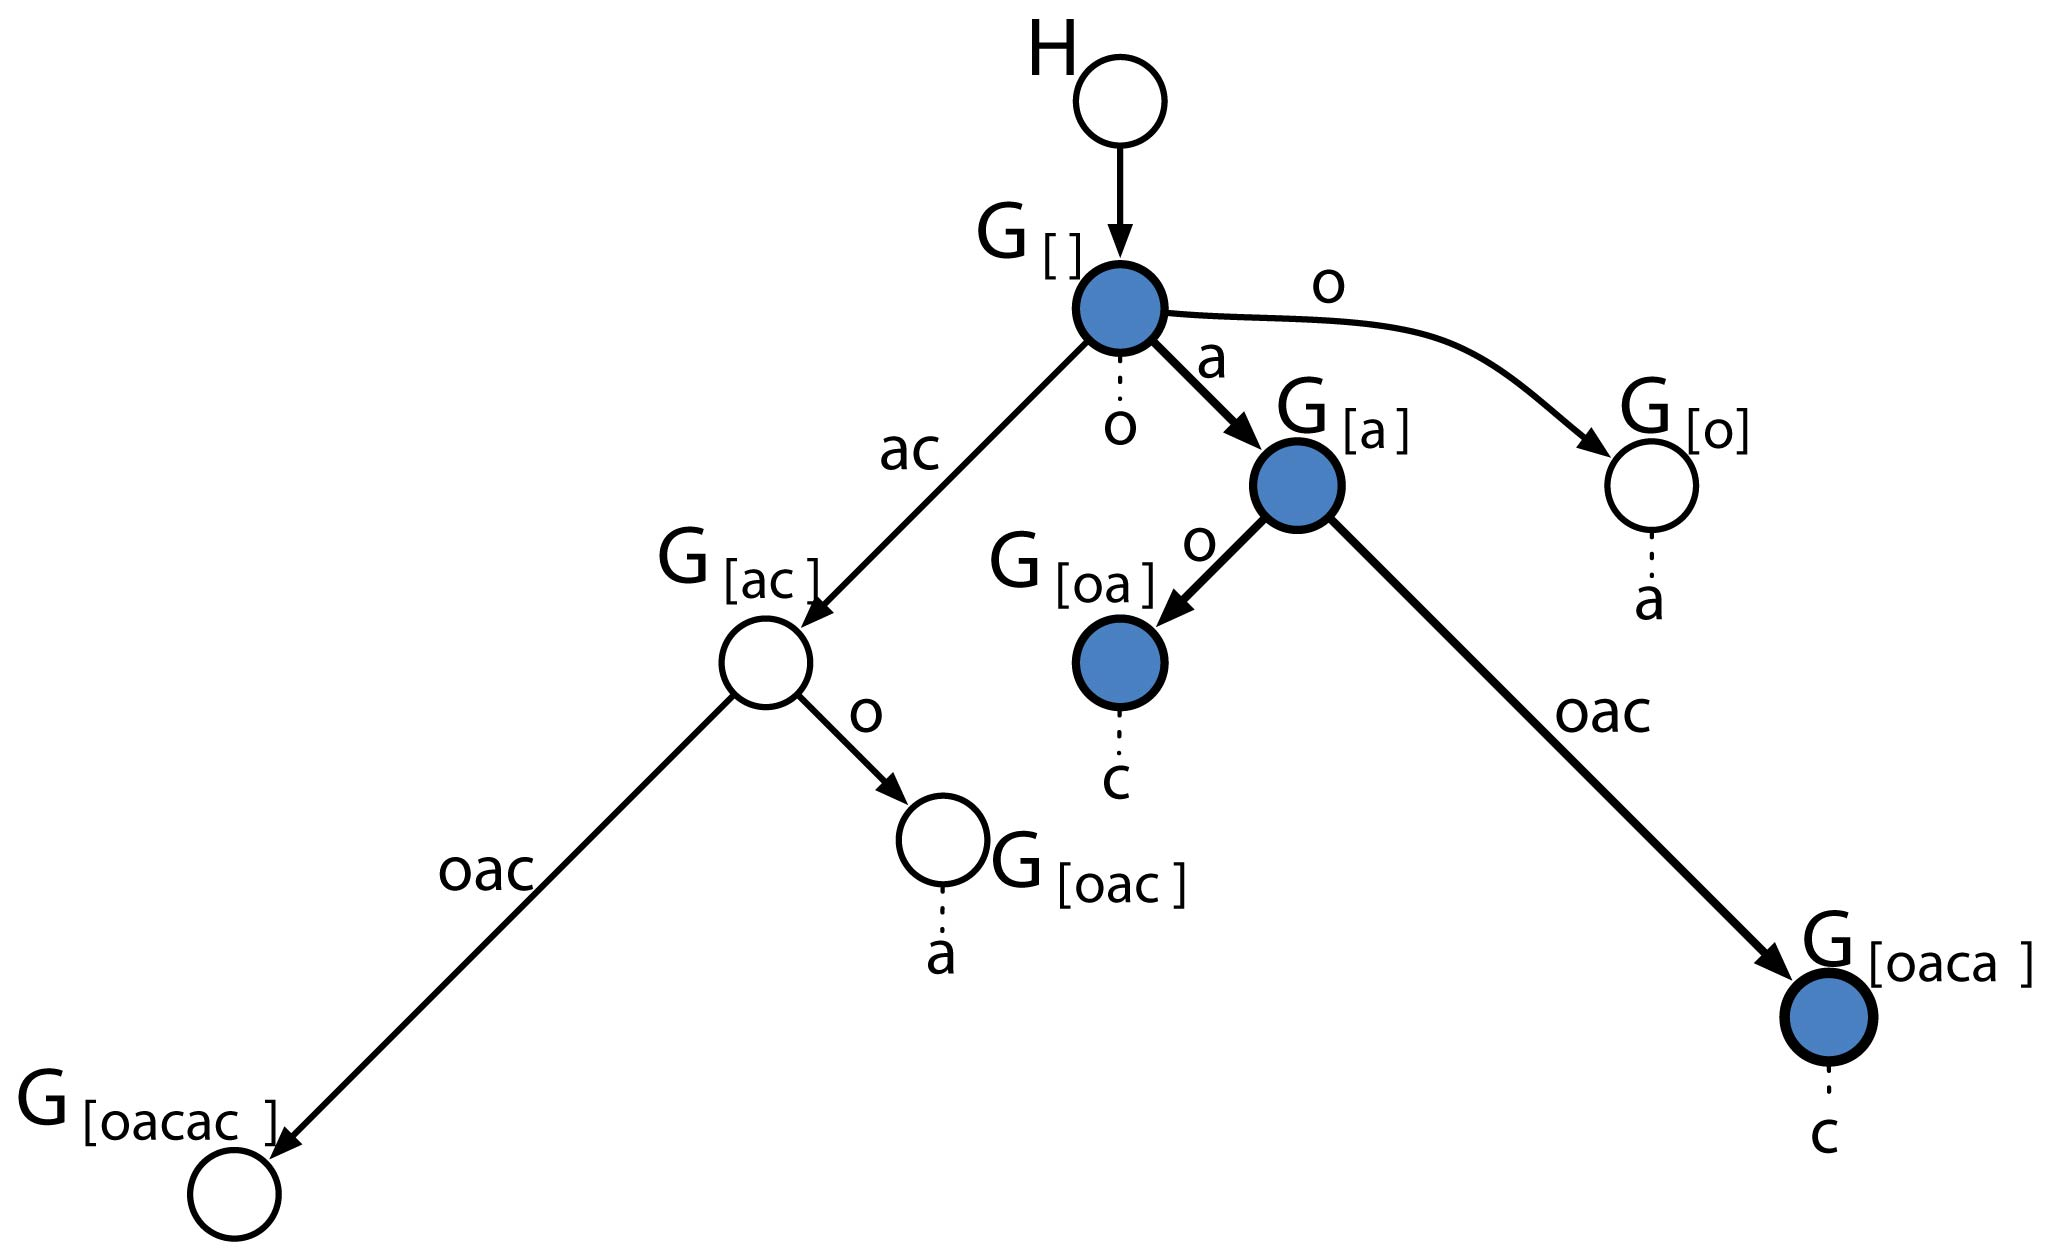
\includegraphics[width=.5\textwidth]{fig/prefix_tree_coloured.pdf}
\caption{Prefix {\em tree} graphical model}
\label{fig: prefix_tree}
\end{center}
\end{figure}
 }
\frame[t] {%slide 22
 \frametitle{}
 }
 \frame[t] {%slide 23
 \frametitle{}
 }
 \frame[t] {%slide 24
 \frametitle{Finite Depth vs.~Infinite Depth - Computational Complexity}
 \begin{figure}[htbp]
\begin{center}
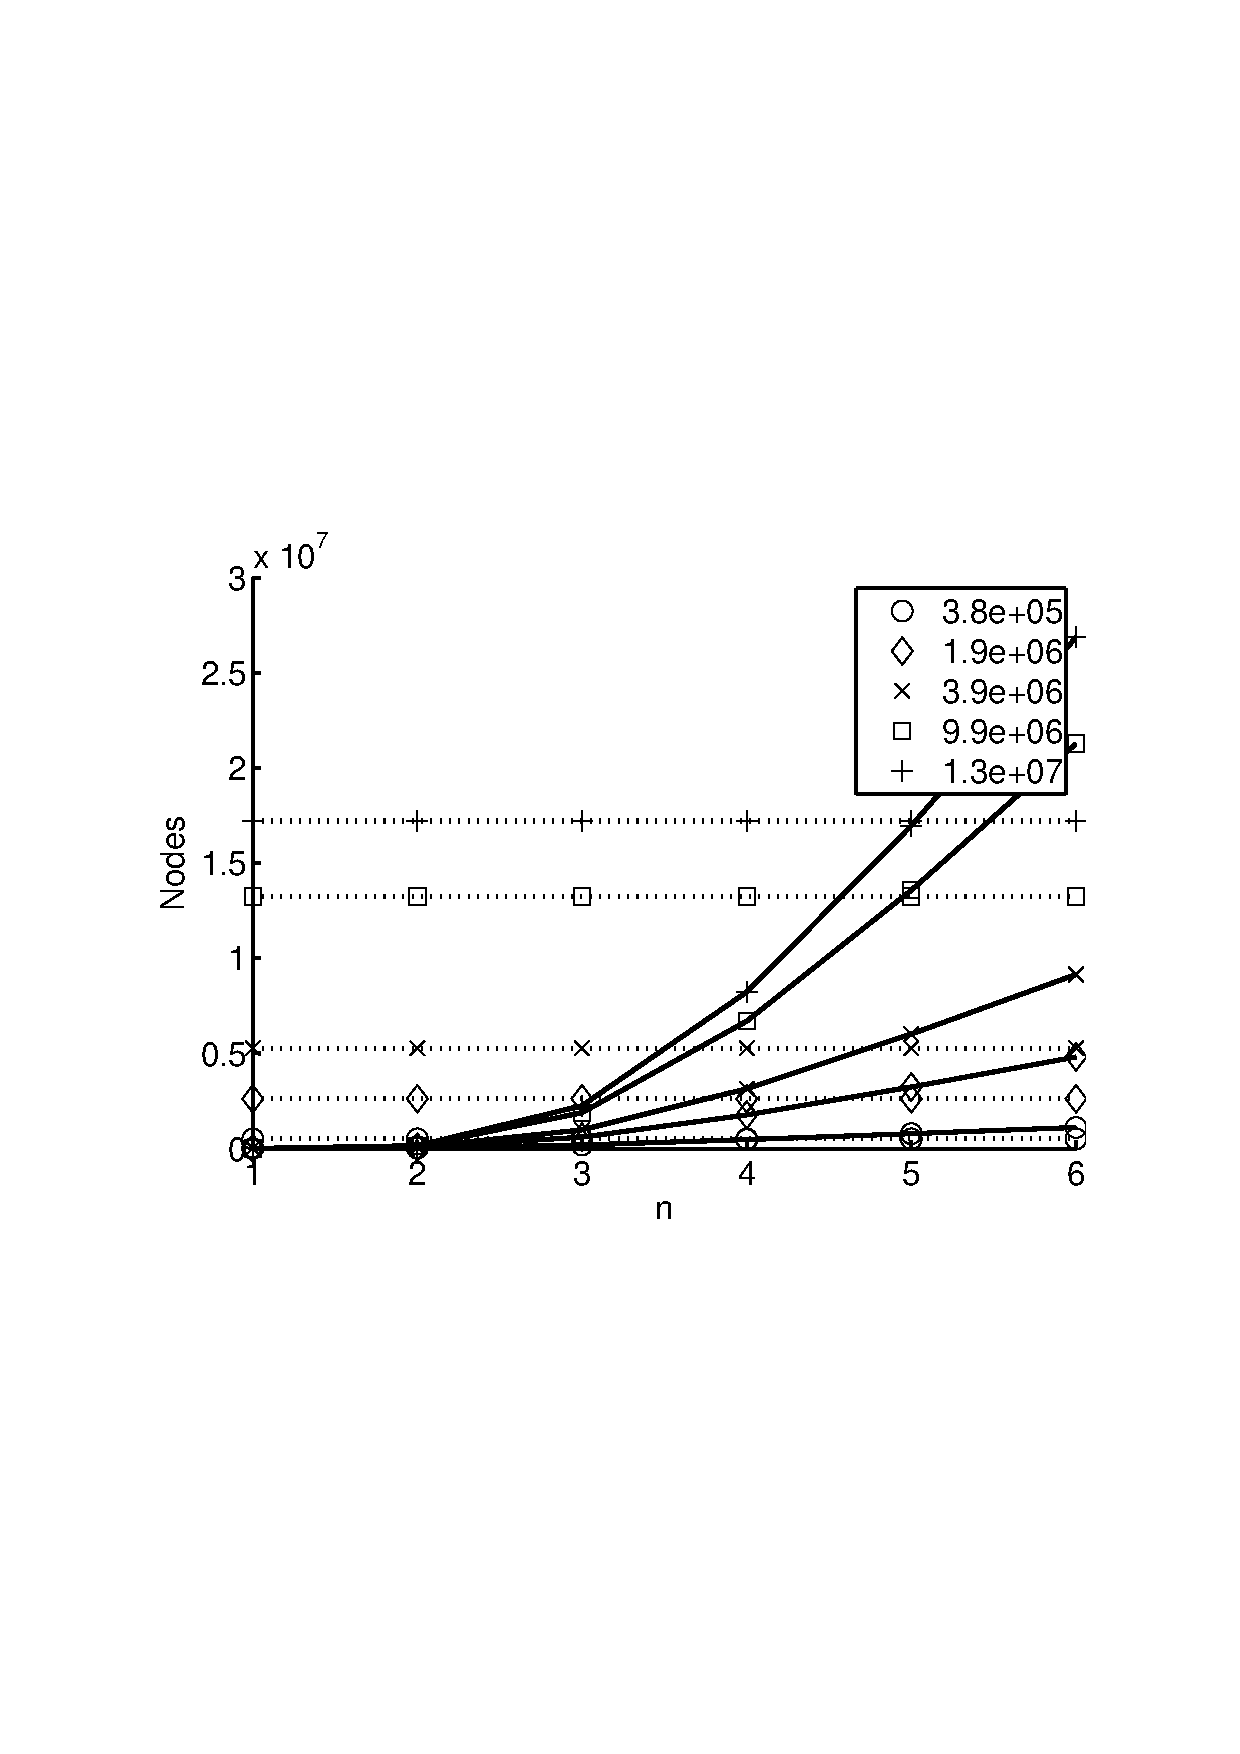
\includegraphics[width=.75\textwidth]{fig/node_counts.pdf}
\caption{Number of nodes vs.~order of Markov model}
\label{fig: node_counts}
\end{center}
\end{figure}
 }
 \frame[t] {%slide 25
 \frametitle{Finite Depth vs.~Infinite Depth - Computational Complexity}
 \begin{figure}[htbp]
\begin{center}
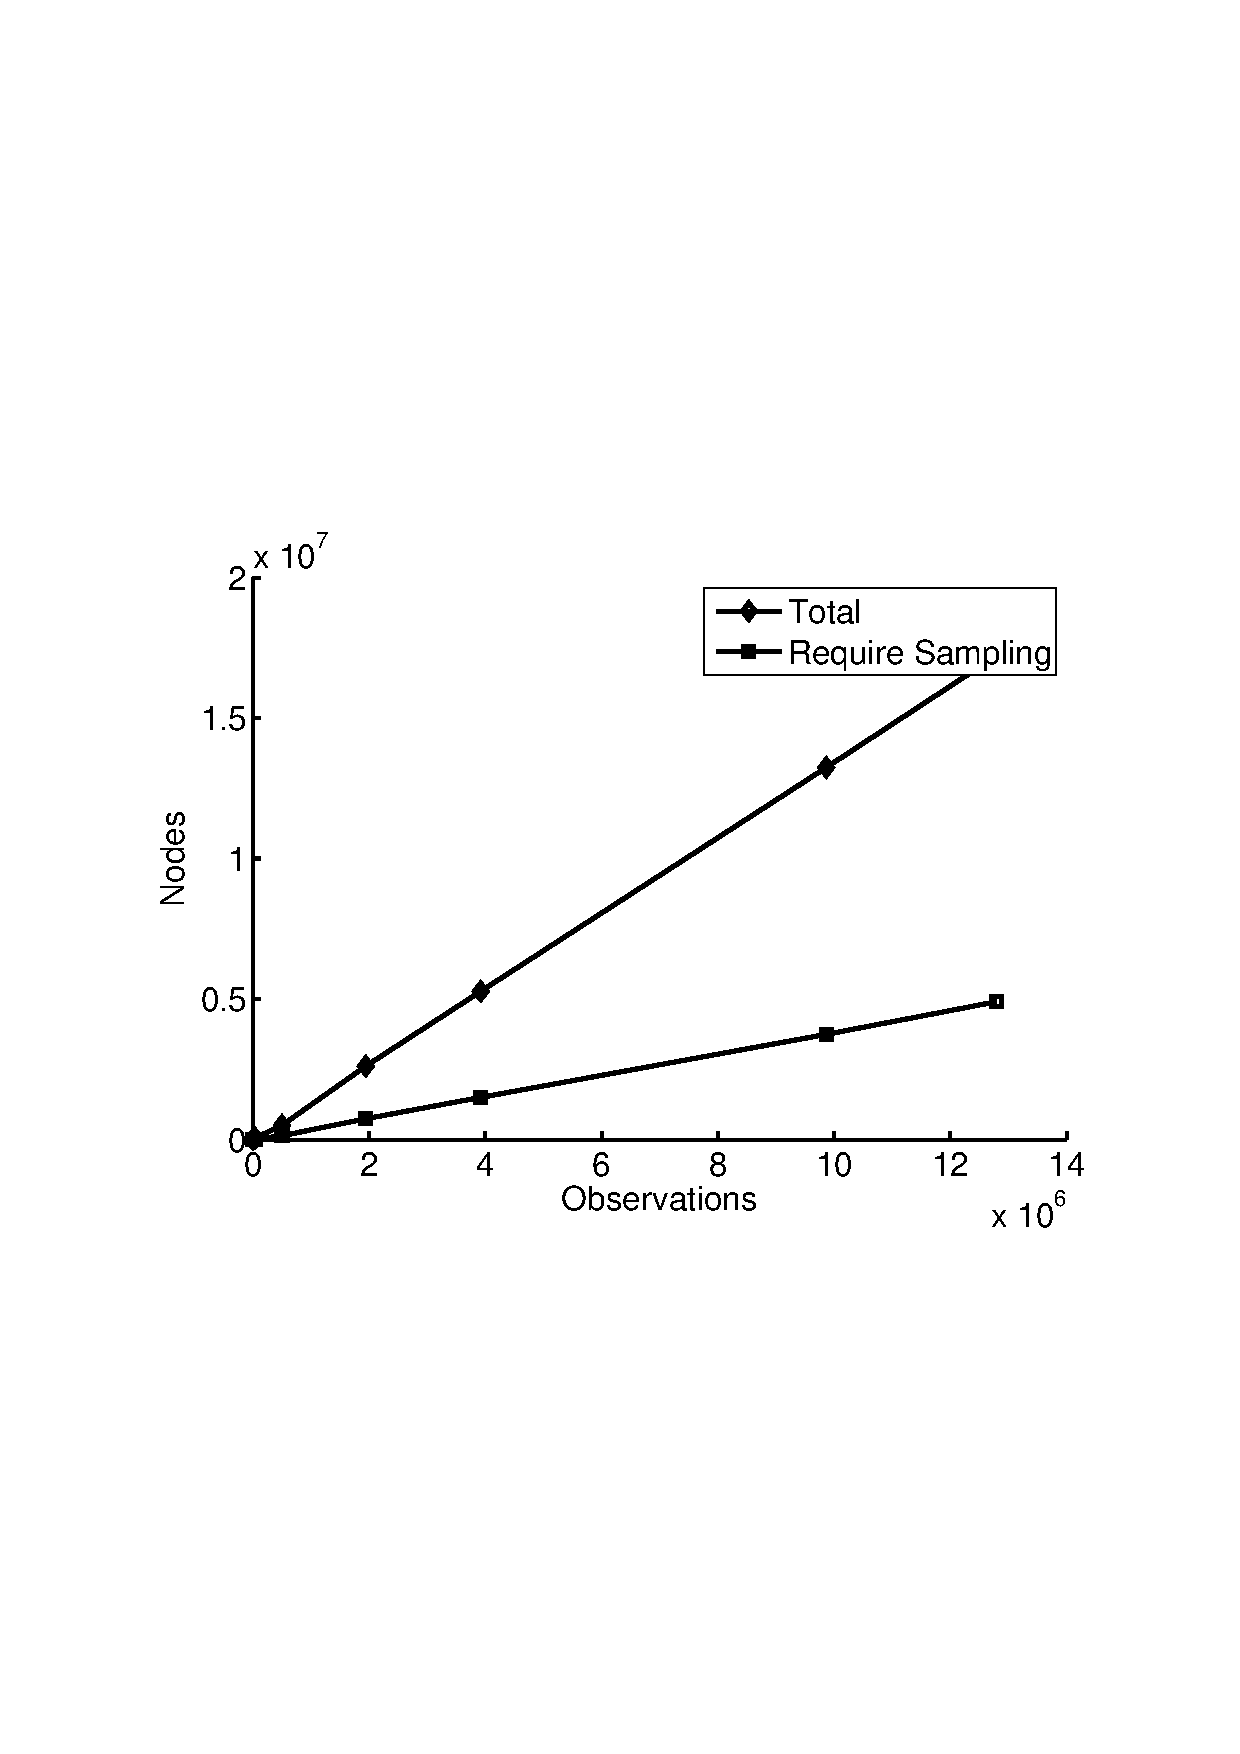
\includegraphics[width=.75\textwidth]{fig/nodes_total_vs_need_sampling.pdf}
\caption{Number of nodes vs.~number of observations}
\label{fig: nodes_total_vs_need_sampling}
\end{center}
\end{figure}
 }
 \frame[t] {%slide 26
 \frametitle{Finite Depth vs.~Infinite Depth - Predictive Power}
 \begin{figure}[htbp]
\begin{center}
\includegraphics[width=.5\textwidth]{fig/fix_size_vary_n_cleaned_coloured.pdf}
\caption{Test perplexity vs.~order of Markov model.}
\label{fig: fix_size_vary_n_cleaned_coloured}
\end{center}
\end{figure}
 }
 \frame[t] {%slide 27
 \frametitle{Finite Depth vs.~Infinite Depth - Predictive Power}
 \begin{figure}[htbp]
\begin{center}
\includegraphics[width=.5\textwidth]{fig/fix_n_vary_size_ap_cleaned_coloured.pdf}
\caption{Test perplexity vs.~number of training observations.}
\label{fig: fix_n_vary_size_ap_cleaned_coloured}
\end{center}
\end{figure}

 }
 \frame[t] {%slide 28
 \frametitle{}
 }
 \frame[t] {%slide 29
 \frametitle{}
 }
 \frame[t] {%slide 30
 \frametitle{}
 }

\bibliographystyle{apalike}
\bibliography{references.bib}

\end{document}
